\begin{figure}
\vspace*{31mm}
\hspace*{72mm}
\begin{tikzpicture}[transform canvas={scale=0.8}]
  \node[font=\itshape\large] (textgg) {\(\forall g\in\{H,X,Y,Z\}\) cancels itself};
  \node[below=-5mm of textgg] (gg) {
    \begin{tikzpicture}
      \node[inner sep=0pt] (c1) at (0,0) {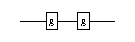
\includegraphics[scale=2]{Figures/circuits/gg}};  
      \node[right=-12mm of c1.east, rectangle, fill=white, minimum size=10mm] (eq) {\(=\)};    
      \node[right=-7mm of eq, inner sep=0pt] (c2) {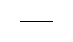
\includegraphics[scale=2]{Figures/circuits/I}};
      \node[right=7mm of c1.west, rectangle,fill=white,minimum size=5mm] {};
      %\node[below right=-1mm and -23mm of eq] (alg) {\small \(g\in\{H,X,Y,Z\}\)};
    \end{tikzpicture}
  };
  \node[above right=28mm and 13mm of textgg, font=\itshape\large] (textCNOT) {CNOT flip};
  \node [below=-5mm of textCNOT] (CNOT) {
    \begin{tikzpicture}
      \node[inner sep=0pt] (c1) at (0,0) {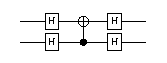
\includegraphics[scale=2]{Figures/circuits/HCNOTH}};       
      \node[right=-13.9mm of c1.east, inner sep=0pt] (c2) {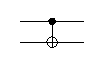
\includegraphics[scale=2]{Figures/circuits/CNOT}};
      \node[right=-12mm of c1.east, rectangle, fill=white, minimum size=10mm] (eq) {\(=\)};  
      \node[right=7mm of c1.west, rectangle,fill=white,minimum width=5mm, minimum height=10mm] {};
      \node[left=7mm of c2.east, rectangle,fill=white,minimum width=5mm, minimum height=10mm] {};
    \end{tikzpicture}
  };
  \node[above left=28mm and 0mm of textgg, font=\itshape\large] (textHXZ) {Rules with \(H\), \(X\), \(Y\) and \(Z\)};
  \node [below left=-5mm and -37mm of textHXZ] (XZ) {
    \begin{tikzpicture}
      \node[inner sep=0pt] (c1) at (0,0) {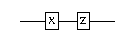
\includegraphics[scale=2]{Figures/circuits/XZ}};       
      \node[below=-3mm of c1] (eq) {\(=\)};  
      \node[below=-3mm of eq, inner sep=0pt] (c2) {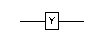
\includegraphics[scale=2]{Figures/circuits/Y}};
      \node[below=-3mm of c2] (eq2) {\(=\)};  
      \node[below=-3mm of eq2, inner sep=0pt] (c3) {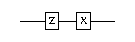
\includegraphics[scale=2]{Figures/circuits/ZX}};
      \node[right=7mm of c1.west, rectangle,fill=white,minimum size=5mm] {};
      \node[left=7mm of c3.east, rectangle,fill=white,minimum size=5mm] {};
      \node[left=7mm of c1.east, rectangle,fill=white,minimum size=5mm] {};
      \node[right=7mm of c3.west, rectangle,fill=white,minimum size=5mm] {};
    \end{tikzpicture}
  };
  \node [below right=-5mm and -37mm of textHXZ] (XH) {
    \begin{tikzpicture}
      \node[inner sep=0pt] (c1) at (0,0) {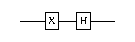
\includegraphics[scale=2]{Figures/circuits/XH}};       
      \node[below=-3mm of c1] (eq) {\(=\)};  
      \node[below=-3mm of eq, inner sep=0pt] (c2) {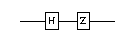
\includegraphics[scale=2]{Figures/circuits/HZ}};
      \node[right=7mm of c1.west, rectangle,fill=white,minimum size=5mm] {};
      \node[left=7mm of c2.east, rectangle,fill=white,minimum size=5mm] {};
      \node[left=7mm of c1.east, rectangle,fill=white,minimum size=5mm] {};
      \node[right=7mm of c2.west, rectangle,fill=white,minimum size=5mm] {};
    \end{tikzpicture}
  };  
  \node[below left=8mm and 7mm of textgg, font=\itshape\large] (textZS) {Rules with \(Z\), \(S\) and \(T\)};
  \node [below left=-5mm and -34mm of textZS] (ZS) {
    \begin{tikzpicture}
      \node[inner sep=0pt] (c1) at (0,0) {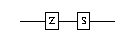
\includegraphics[scale=2]{Figures/circuits/ZS}};       
      \node[below=-3mm of c1] (eq) {\(=\)};  
      \node[below=-3mm of eq, inner sep=0pt] (c2) {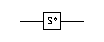
\includegraphics[scale=2]{Figures/circuits/S'}};
      \node[right=7mm of c1.west, rectangle,fill=white,minimum size=5mm] {};
      \node[left=7mm of c1.east, rectangle,fill=white,minimum size=5mm] {};
    \end{tikzpicture}
  };
  \node [below right=-5mm and -34mm of textZS] (ZT) {
    \begin{tikzpicture}
      \node[inner sep=0pt] (c1) at (0,0) {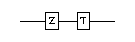
\includegraphics[scale=2]{Figures/circuits/ZT}};       
      \node[below=-3mm of c1] (eq) {\(=\)};  
      \node[below=-3mm of eq, inner sep=0pt] (c2) {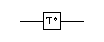
\includegraphics[scale=2]{Figures/circuits/T'}};
      \node[right=7mm of c1.west, rectangle,fill=white,minimum size=5mm] {};
      \node[left=7mm of c1.east, rectangle,fill=white,minimum size=5mm] {};
    \end{tikzpicture}
  };
  \node[below right=8mm and 3mm of textgg, font=\itshape\large] (textXS) {Rules with \(X\), \(S\) and \(T\)};
  \node [below left=-5mm and -34mm of textXS] (XS) {
    \begin{tikzpicture}
      \node[inner sep=0pt] (c1) at (0,0) {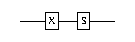
\includegraphics[scale=2]{Figures/circuits/XS}};       
      \node[below=-3mm of c1] (eq) {\(=\)};  
      \node[below=-3mm of eq, inner sep=0pt] (c2) {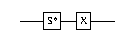
\includegraphics[scale=2]{Figures/circuits/SX}};
      \node[right=7mm of c1.west, rectangle,fill=white,minimum size=5mm] {};
      \node[left=7mm of c2.east, rectangle,fill=white,minimum size=5mm] {};
      \node[left=7mm of c1.east, rectangle,fill=white,minimum size=5mm] {};
      \node[right=7mm of c2.west, rectangle,fill=white,minimum size=5mm] {};
    \end{tikzpicture}
  };
  \node [below right=-5mm and -34mm of textXS] (XT) {
    \begin{tikzpicture}
      \node[inner sep=0pt] (c1) at (0,0) {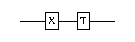
\includegraphics[scale=2]{Figures/circuits/XT}};       
      \node[below=-3mm of c1] (eq) {\(=\)};  
      \node[below=-3mm of eq, inner sep=0pt] (c2) {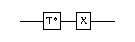
\includegraphics[scale=2]{Figures/circuits/TX}};
      \node[right=7mm of c1.west, rectangle,fill=white,minimum size=5mm] {};
      \node[left=7mm of c2.east, rectangle,fill=white,minimum size=5mm] {};
      \node[left=7mm of c1.east, rectangle,fill=white,minimum size=5mm] {};
      \node[right=7mm of c2.west, rectangle,fill=white,minimum size=5mm] {};
    \end{tikzpicture}
  };
\end{tikzpicture}
\vspace*{35mm}
\caption{Some basic properties of the gates in the Clifford+T set. Here, \(S^*\) and \(T^*\) represent the inverse gates of \(S\) and \(T\), i.e. their conjugate transpose, usually written as \(S^\dag\) and \(T^\dag\).}
\label{fig:props}
\end{figure}